\documentclass[slovene,11pt,a4paper]{article}
%\usepackage{fullpage}
\usepackage[margin=2cm]{geometry}

\usepackage[T1]{fontenc}



%dodatni paketki:
\usepackage{graphicx}
\usepackage{amsmath,amsfonts,amsthm} %matematicni paket
\usepackage{color} % omogoča barvno pisanje
\usepackage[utf8]
{inputenc}
\usepackage[slovene]{babel} % slovenski jezik/hyphenation
\usepackage{hyperref} %naredi vse povezave rečerenc, kazala,...
\numberwithin{equation}{section} % Number equations within sections (i.e. 1.1, 1.2, 2.1, 2.2 instead of 1, 2, 3, 4)
\numberwithin{figure}{section} % Number figures within sections (i.e. 1.1, 1.2, 2.1, 2.2 instead of 1, 2, 3, 4)
\numberwithin{table}{section} % Number tables within sections (i.e. 1.1, 1.2, 2.1, 2.2 instead of 1, 2, 3, 4)
\usepackage{eurosym} %za znak €

\usepackage{mathrsfs}
\usepackage{mathabx} % za kemisjke smeri in naslednje 3 vstrice
\catcode`_=12
\begingroup\lccode`~=`_\lowercase{\endgroup\let~\sb}
\mathcode`_="8000

\usepackage{placeins}
\usepackage[margin=2cm]{geometry}



\begin{document}
\begin{titlepage}

\newcommand{\HRule}{\rule{\linewidth}{0.5mm}} % Defines a new command for the horizontal lines, change thickness here

\center % Center everything on the page

%----------------------------------------------------------------------------------------
%	LOGO
%----------------------------------------------------------------------------------------

%\includegraphics{Logo}\\[1cm] % Include a department/university logo - this will require the graphicx package
 
%----------------------------------------------------------------------------------------


\includegraphics[width=2cm]{slike/aaa}\\[0.5cm]
 
%----------------------------------------------------------------------------------------
%	NASLOV DELA
%----------------------------------------------------------------------------------------
\textit{Univerza v Ljubljani}\\
\textit{Fakulteta za {\color{red}matematiko in fiziko}}\\[0.5cm]

\emph{Oddelek za fiziko}\\[0.5cm] % Oddelek za fiziko


%----------------------------------------------------------------------------------------
%	TITLE SECTION
%--------------------------------------------------------------------------------------
\HRule \\[0.4cm]
\huge {\bfseries 2. naloga: Trotter-suzuki razcep -1.del}\\[0.4cm] % NASLOV SEMINARJA
\HRule \\[0.5cm] 

 \textsc{\large Poročilo pri predmetu višje računske metode}\\
 \textsc{\large 2016/2017}\\[1cm] % SEMINASKO DELO
 
%----------------------------------------------------------------------------------------
%	AUTHOR SECTION
%----------------------------------------------------------------------------------------



% If you don't want a supervisor, uncomment the two lines below and remove the section above
\Large \emph{Avtor:}\\
Klemen \textsc{Rahne}\\
28152028\\[2cm]
%----------------------------------------------------------------------------------------
%	DATUM
%----------------------------------------------------------------------------------------

{\large \today } \\[0.5cm] % Date, change the \today to a set date if you want to be precise

	

\end{titlepage}


%----------------------------------------------------------------------------------------
%	KAZALO
%----------------------------------------------------------------------------------------

%\tableofcontents

%----------------------------------------------------------------------------------------
%	ZAČETEK TEKSTA
%----------------------------------------------------------------------------------------
\section{naloga}

Imamo Hamiltonko H, ki opisuje delec v harmonskem potencialu v dveh dimenzijah:

\begin{equation}
\label{hamiltonka}
H =  \frac{1}{2} p_1^2 +\frac{1}{2} p_2^2 + \frac{1}{2} q_1^2 +\frac{1}{2} q_2^2 + \lambda q_1^2 q_2^2
\end{equation}
Oglejmo si nekaj trajektorij delcev z različnimi vrednostmi $\lambda$. Trajektorije smo reševali s Trotter-Suzuki algoritmom.


\begin{figure}[!htb]
\centering
\begin{minipage}{0.5\textwidth}
\centering
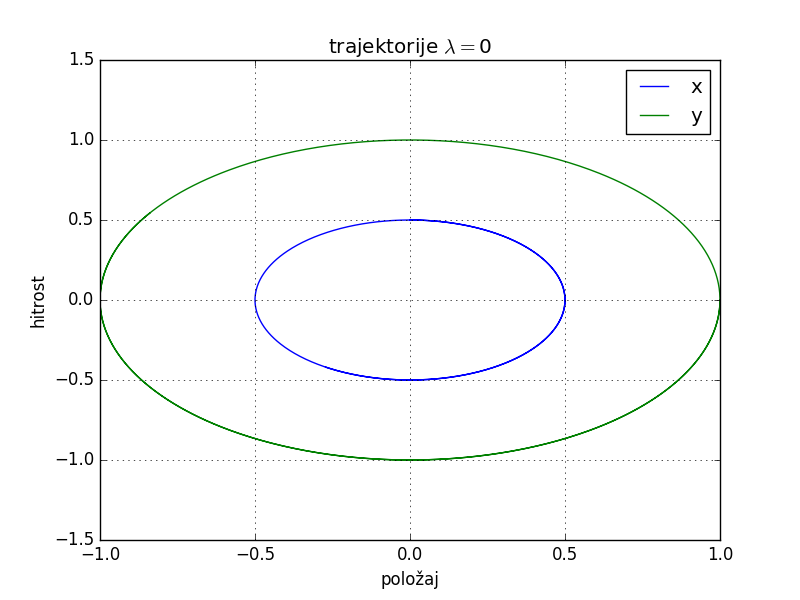
\includegraphics[scale=0.45]{slike/trajektorije_0.png}
%\caption{first figure}
\end{minipage}\hfill
\begin{minipage}{0.5\textwidth}
\centering
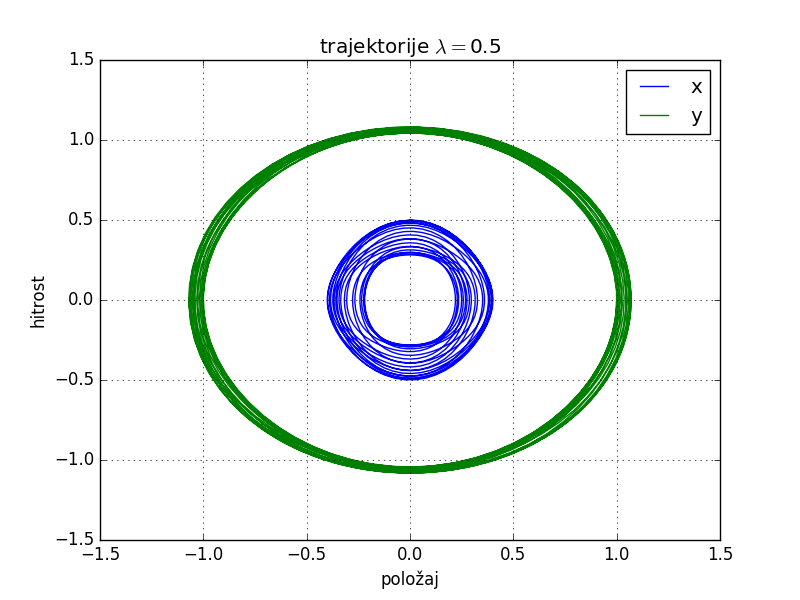
\includegraphics[scale=0.45]{slike/trajektorije_1.png}
%\caption{second figure}
\end{minipage}

\caption{Značilne trajektorije za Hamiltonko \ref{hamiltonka} z začetnimo pogoji $(q_1,p_1,q_2,p_2)=(0,\frac{1}{2},1,0)$. Pri $\lambda=0$ se vidi, kot da imamo dva neodvisna harmonska oscilatorja. Z vključitvijo dodatnega člena ($\lambda q_1^2 q_2^2$), se trajektorije v posamezni dimenziji spremenijo. }
\end{figure}


\begin{figure}[!htb]
\centering
\begin{minipage}{0.5\textwidth}
\centering
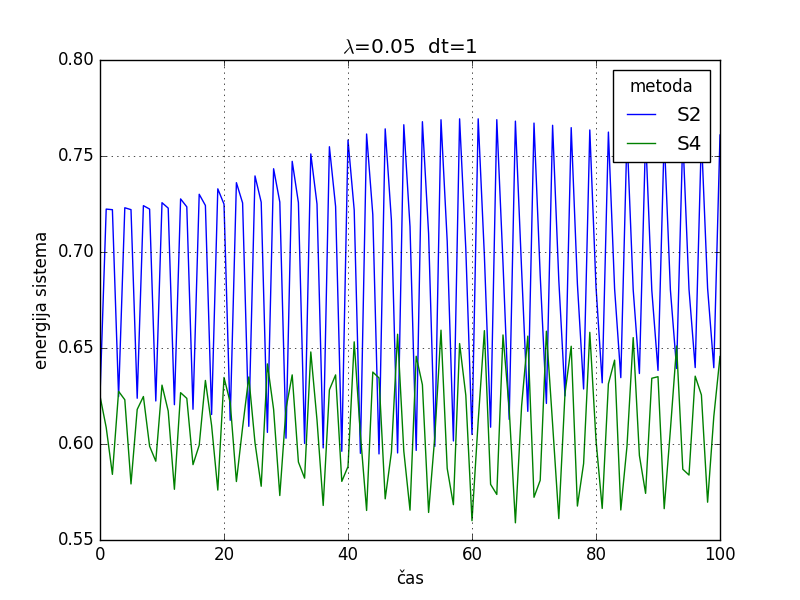
\includegraphics[scale=0.45]{slike/energija_0_1.png}
%\caption{first figure}
\end{minipage}\hfill
\begin{minipage}{0.5\textwidth}
\centering
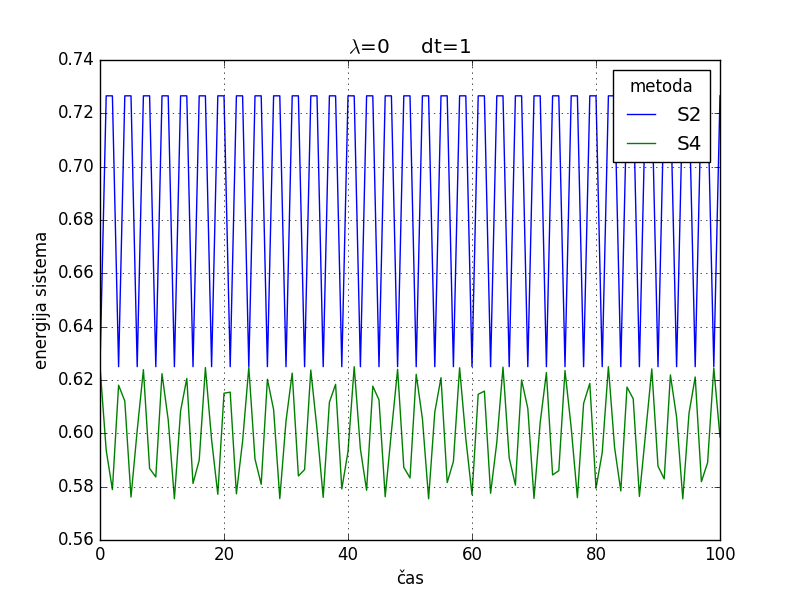
\includegraphics[scale=0.45]{slike/energija_0_2.png}
%\caption{second figure}
\end{minipage}

\caption{Ohranjanje energije pri dveh različnim metodah-S2 in S4. Opazimo precejšnje oscilacije okoli stacionarne lege, ki pa sta različni od začetne energije.Pri višjih vrednostih $\lambda$ postane metoda S4 nestabilna.}
\end{figure}


\begin{figure}[!ht]
\centering
\begin{minipage}{0.5\textwidth}
\centering
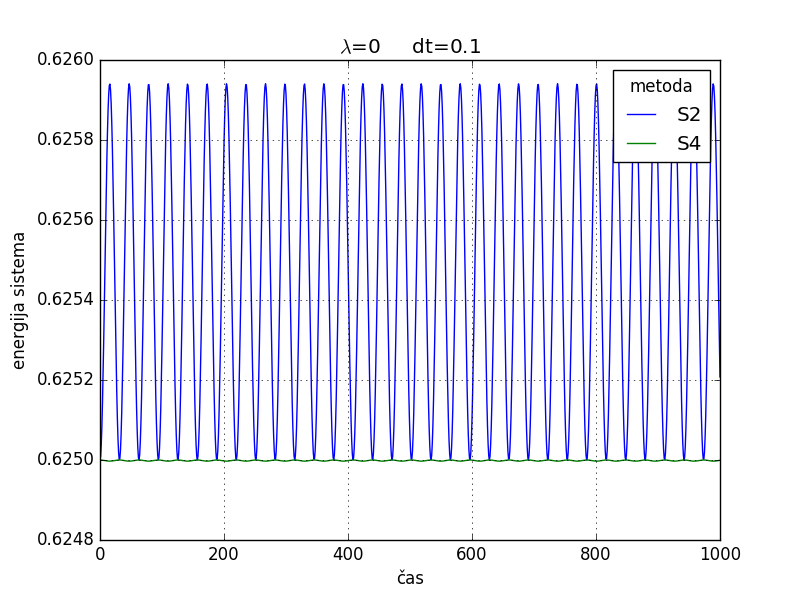
\includegraphics[scale=0.45]{slike/energija_1_1.png}
%\caption{first figure}
\end{minipage}\hfill
\begin{minipage}{0.5\textwidth}
\centering
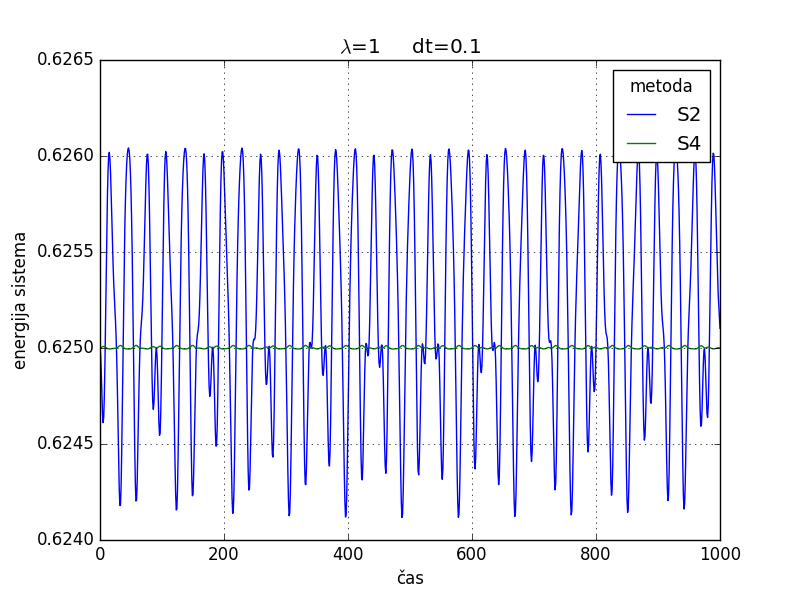
\includegraphics[scale=0.45]{slike/energija_1_2.png}
%\caption{second figure}
\end{minipage}
\caption{Pri manjšanju časovnega intervala se pri metodi S4 oscilacije zmanjšajo na , ter zavzema energijo iz začetnih pogojev. Metoda S2 ponovno oscilira, vendar z manjšo amplitudo. Tudi tokrat ima ta metoda v povprečju večjo energijo od začetne vrednost.}
\end{figure}


\FloatBarrier

\section{Ekviparticijski teorem}
Ekviparticijski teorem pravi, da se energija sistema v termodinamskem ravnovesju enakomerno porazdeli med vse tipe energij sistema (kinetična, potencialna) in med prostostnimi stopnjami. To bomo preverili z vrednostjo
\begin{equation}
\langle p_i^2 \rangle (t) = \frac{1}{t} \int_0^t p_j^2 (t') dt'
\end{equation}
ki predstavlja kinetično energijo v $i$ti smeri.

\begin{figure}[!ht]
\centering
\begin{minipage}{0.5\textwidth}
\centering
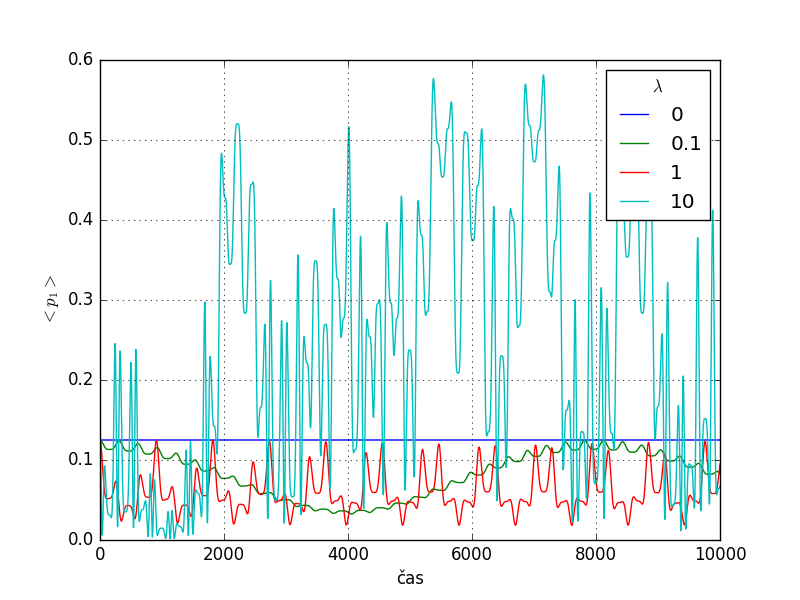
\includegraphics[scale=0.45]{slike/ekviparticija1.png}
%\caption{first figure}
\end{minipage}\hfill
\begin{minipage}{0.5\textwidth}
\centering
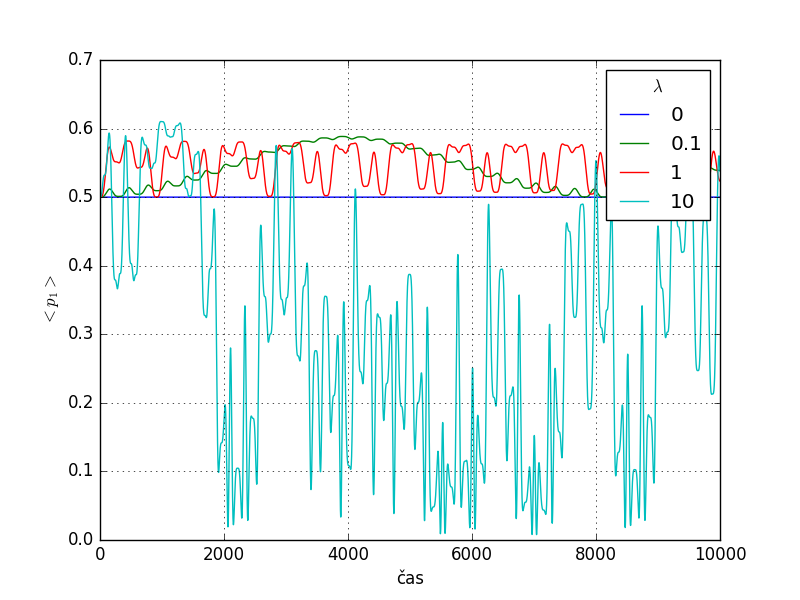
\includegraphics[scale=0.45]{slike/ekviparticija2.png}
%\caption{second figure}
\end{minipage}
\caption{Levo:$\langle p_1^2 \rangle (t) $, desno: $\langle p_2^2 \rangle (t)$. Opazimo, da v primeru večanja parametra $\lambda$ imamo bolj nepredvidljive vrednosti povprečne vrednosti hitrosti na kvadrat, kar nam nakazuje da se približujemo bolj statističnem opisu gibanja-oz. ekviparticijkem teoremu.}
\end{figure}



\end{document}
